% !TeX root = ../../main.tex

\subsection{Transferring from 2-DOF to 3-DOF Arm Environment}

Moving to new physics engine where it's possible to design more complex environment and to experiment the transferibility between physics engines, how we can use trained agent to do more complex tasks in different environment, how the agent will behave in such an environment, whether the agent will need to be trained from the beginning or it will be able to perform the task and maximize the average return for accomplishing the goal of the environment.


This experiment is performed on a different physics engine (Unity MLAgents) which provide more complex environment and allows the environment to have multiple agent inside it which provide parallel training in one environment.

\subsubsection{Aim of the experiment}
% 1. Question behind (in the heading, why interesting, what to investigate)

This experiment is conducted multiple times with different purposes to experemnt new approach and compare between existing reinforcement learning physics engines to show the performace, training time and the advantages of each engine.

The first trail of the experiment was conducted to train the agents from scratch using the same algorithms used in pervouis experiment. In this way, it's possible to compare between the two physics engine, how the agent behave in each of the environment, whether it's better to have multiple agent living inside a single environment to train them or to parallelize the environemnt to have multiple instance of the environemtn to perform the training. 

In the second trail, a new training for the 3rd experiment is conducted with a new neural network which shares the same observation and action spaces of the unity environment. The trained agent will be tested and evaluated on the unity environment to evaluate the agent behaviour and test if it's possible to transfer learning between two environment sharing the same observation and action spaces. In this experiment, we investage how can we benefit from trained agent and reuse it in different environemtn to acheive a specific goal, whether the agent will perform the task successfully or it will need to continue exploring the environment and continue some training in the new environemnt to reach the goal and maximize the average return.

\subsubsection{Setup and configurations}

In this section we describe the setup of the experiment and how it was performed. Firstly, we introduce and describe the new designed unity environemt. Then, based on the environment description, we present the observation space, action space and reward function of the experiment as a base towards the learning process and achieving environment goal. Subsequently, we describe the learning process. For this, we present the reinforcement learning algorithm and neural network architecture used.


\subsubsection{Environment Description: 3-DOF Robotic Arm}

The new environemt~\ref{fig:unity_environment} consist of double-jointed arm which can move in a 3D space inside the environemtn. The arm is placed in a squared zone where the arm is connected to a point and can move freely in the xyz axes. Inside the environemnt, a moving target sphere which moves in a circular path around the robotic arm and have a moving speed which increase in time. The goal of the agent is to move its hand to reach the moving sphere and keep following the sphere path while it's moving in the environment.

In this environment, it's possible to have multiple agent in the same environment to enable parallization inside the environemnt itself. In this way, the environment contains \textbf{20 agent} linked to a single Brain. The brain is responsible for deciding which actions each of its linked agents will take as descriped in subsection~\ref{unity_mlagents}. In the following figure, a visual photo for the used environment with the 20 agent.

\begin{figure}[!htb]
		\centering
				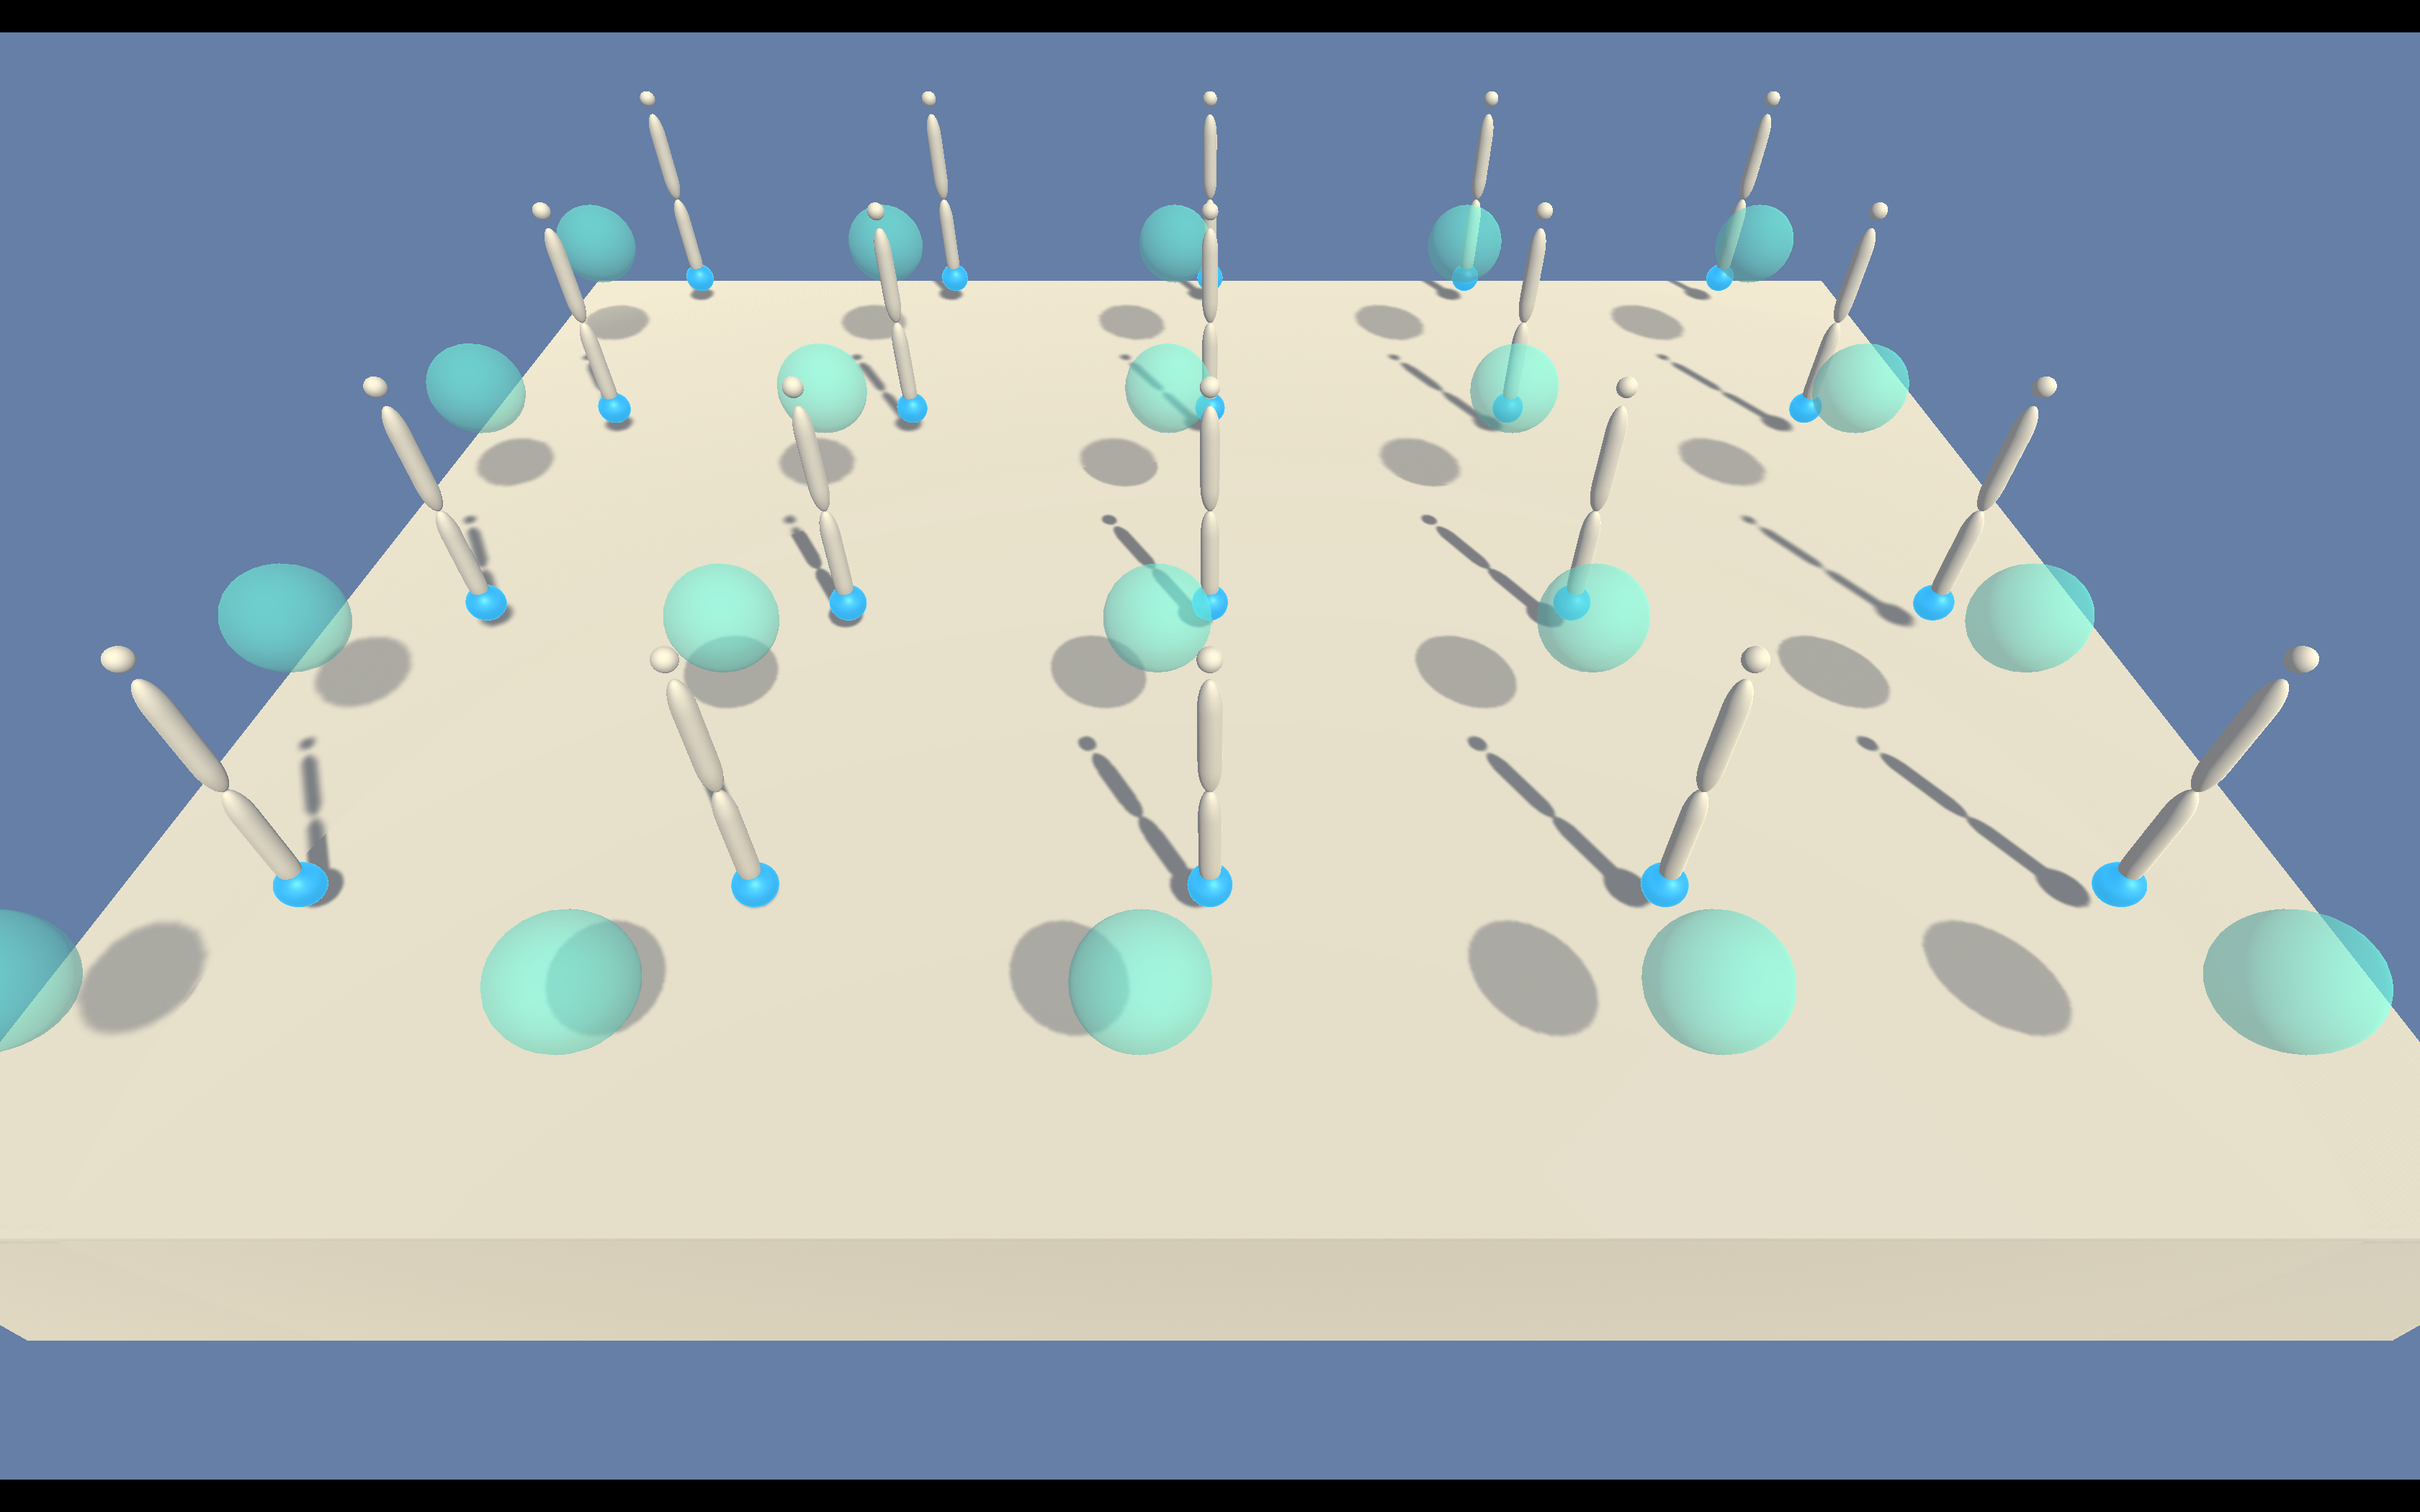
\includegraphics[width=\linewidth]{figures/envs/unity_reacher_20.png}
				\caption{3D Robotic Arm Unity Environment}
				\label{fig:unity_environment}
\end{figure}

\subsubsection{Observation Space}

The observation space of the environment consist of 26 variables corresponding to position, rotation, velocity, and angular velocities of the two arm Rigidbodies. In the following table~\ref{tab:unity_obs_space}, a full description for all the environemt observation is provided.

\begin{table}[!htb]
		\centering
		\begin{tabular}{|c|l|l|c|}
				\hline
				\multicolumn{4}{|c|}{\textbf{Observation Space}}                                                                                                                                     \\ \hline
				\multicolumn{3}{|c|}{\textit{\textbf{pendulumA.transform.localPosition}}} & \textit{X-Axis, Y-Axis, Z-Axis}                                                                          \\ \hline
				\multicolumn{3}{|c|}{\textit{\textbf{pendulumA.transform.rotation}}}      & \textit{X-Axis, Y-Axis, Z-Axis}                                                                          \\ \hline
				\multicolumn{3}{|c|}{\textit{\textbf{rbA.angularVelocity}}}               & \textit{\begin{tabular}[c]{@{}c@{}}how fast an object rotates\\  relative to another point\end{tabular}} \\ \hline
						\multicolumn{3}{|c|}{\textit{\textbf{rbA.velocity}}}                      & \textit{the speed of the arm}                                                                            \\ \hline
				\multicolumn{3}{|c|}{\textit{\textbf{pendulumA.transform.localPosition}}} & \textit{X-Axis, Y-Axis, Z-Axis}                                                                          \\ \hline
				\multicolumn{3}{|c|}{\textit{\textbf{pendulumA.transform.rotation}}}      & \textit{X-Axis, Y-Axis, Z-Axis}                                                                          \\ \hline
				\multicolumn{3}{|c|}{\textit{\textbf{rbB.angularVelocity}}}               & \textit{\begin{tabular}[c]{@{}c@{}}how fast an object rotates\\  relative to another point\end{tabular}} \\ \hline
						\multicolumn{3}{|c|}{\textit{\textbf{rbB.velocity}}}                      & \textit{the speed of the arm}                                                                            \\ \hline
				\multicolumn{3}{|c|}{\textit{\textbf{goal.transform.localPosition}}}      & \textit{X-Axis, Y-Axis, Z-Axis}                                                                          \\ \hline
				\multicolumn{3}{|c|}{\textit{\textbf{hand.transform.localPosition}}}      & \textit{X-Axis, Y-Axis, Z-Axis}                                                                          \\ \hline
				\multicolumn{3}{|c|}{\textit{\textbf{goalSpeed}}}                         & \textit{The speed of the target sphere}                                                                  \\ \hline
		\end{tabular}
		\caption{Unity Observation Space}
		\label{tab:unity_obs_space}
\end{table}

\subsubsection{Action Space}

The action space of the environment is a continuous one in which it has a vector of 4 actions applied to the two joints which indicated the torque applied on the movement axes in the 3D space.


\begin{table}[!htb]
		\centering

		\begin{tabular}{|c|c|l|l|}
				\hline
				\multicolumn{4}{|c|}{\textbf{Action Space (Continuous)}}                                                    \\ \hline
				\multirow{2}{*}{\textbf{Center Joint Torques}}  & \multicolumn{3}{c|}{\textbf{torque X-axis: range(-1, 1)}} \\ \cline{2-4} 
																										& \multicolumn{3}{c|}{\textbf{torque Z-axis: range(-1, 1)}} \\ \hline
				\multirow{2}{*}{\textbf{Elbow Joint Torques}}   & \multicolumn{3}{c|}{\textbf{torque X-axis: range(-1, 1)}} \\ \cline{2-4} 
																										& \multicolumn{3}{c|}{\textbf{torque Z-axis: range(-1, 1)}} \\ \hline
		\end{tabular}
		\caption{Unity 3D Arm Actions Information}
		\label{tab:unity_arm_actions}

\end{table}

\subsubsection{Reward Function}

The reward function is designed to enable the arm to follow the moving sphere as much as possible as it only provide a (+0.1) reward for each step the agent's hand is in goal location. 


\subsubsection{Experiment Results}

$\bullet$ \textit{First Trail: Training from scartch} in this experiment, we trained the agents from scartch to observe the behaviour of training multiple agents inside one environemnt and to compare the training process of unity engine with openai gym (pybullet physics engine). 

The experiment is performed until an average reward of 21 achieved or for a maximum of 10000000 (10M) steps if no improvement is observable. For evaluating the model performance, we compare the average reward between both experiments. In total, we measure the following metrics averaging over each episode:
\begin{itemize}
		\item The Maximum reward the agent can achieve
		\item The Average reward the agent can achieve
		\item The Total Time Steps obtained by the agent
		\item The Total Time taken to perform the experiment
\end{itemize}

Starting from the maximum reward the agent has obtained, we observe that the agent could quickly learn how to reach the target sphere after only 1M time-steps, passing the non-distributed agent score. After 4M time-steps, the agent achieve the maximum reward (40) that can be obtained in the environment. In the following figure~\ref{fig:3rd_exp_max_eps_reward}, the performance of both the agent for the maximum reward in the environment is shown below:
\begin{figure}[!htb]
		\centering
		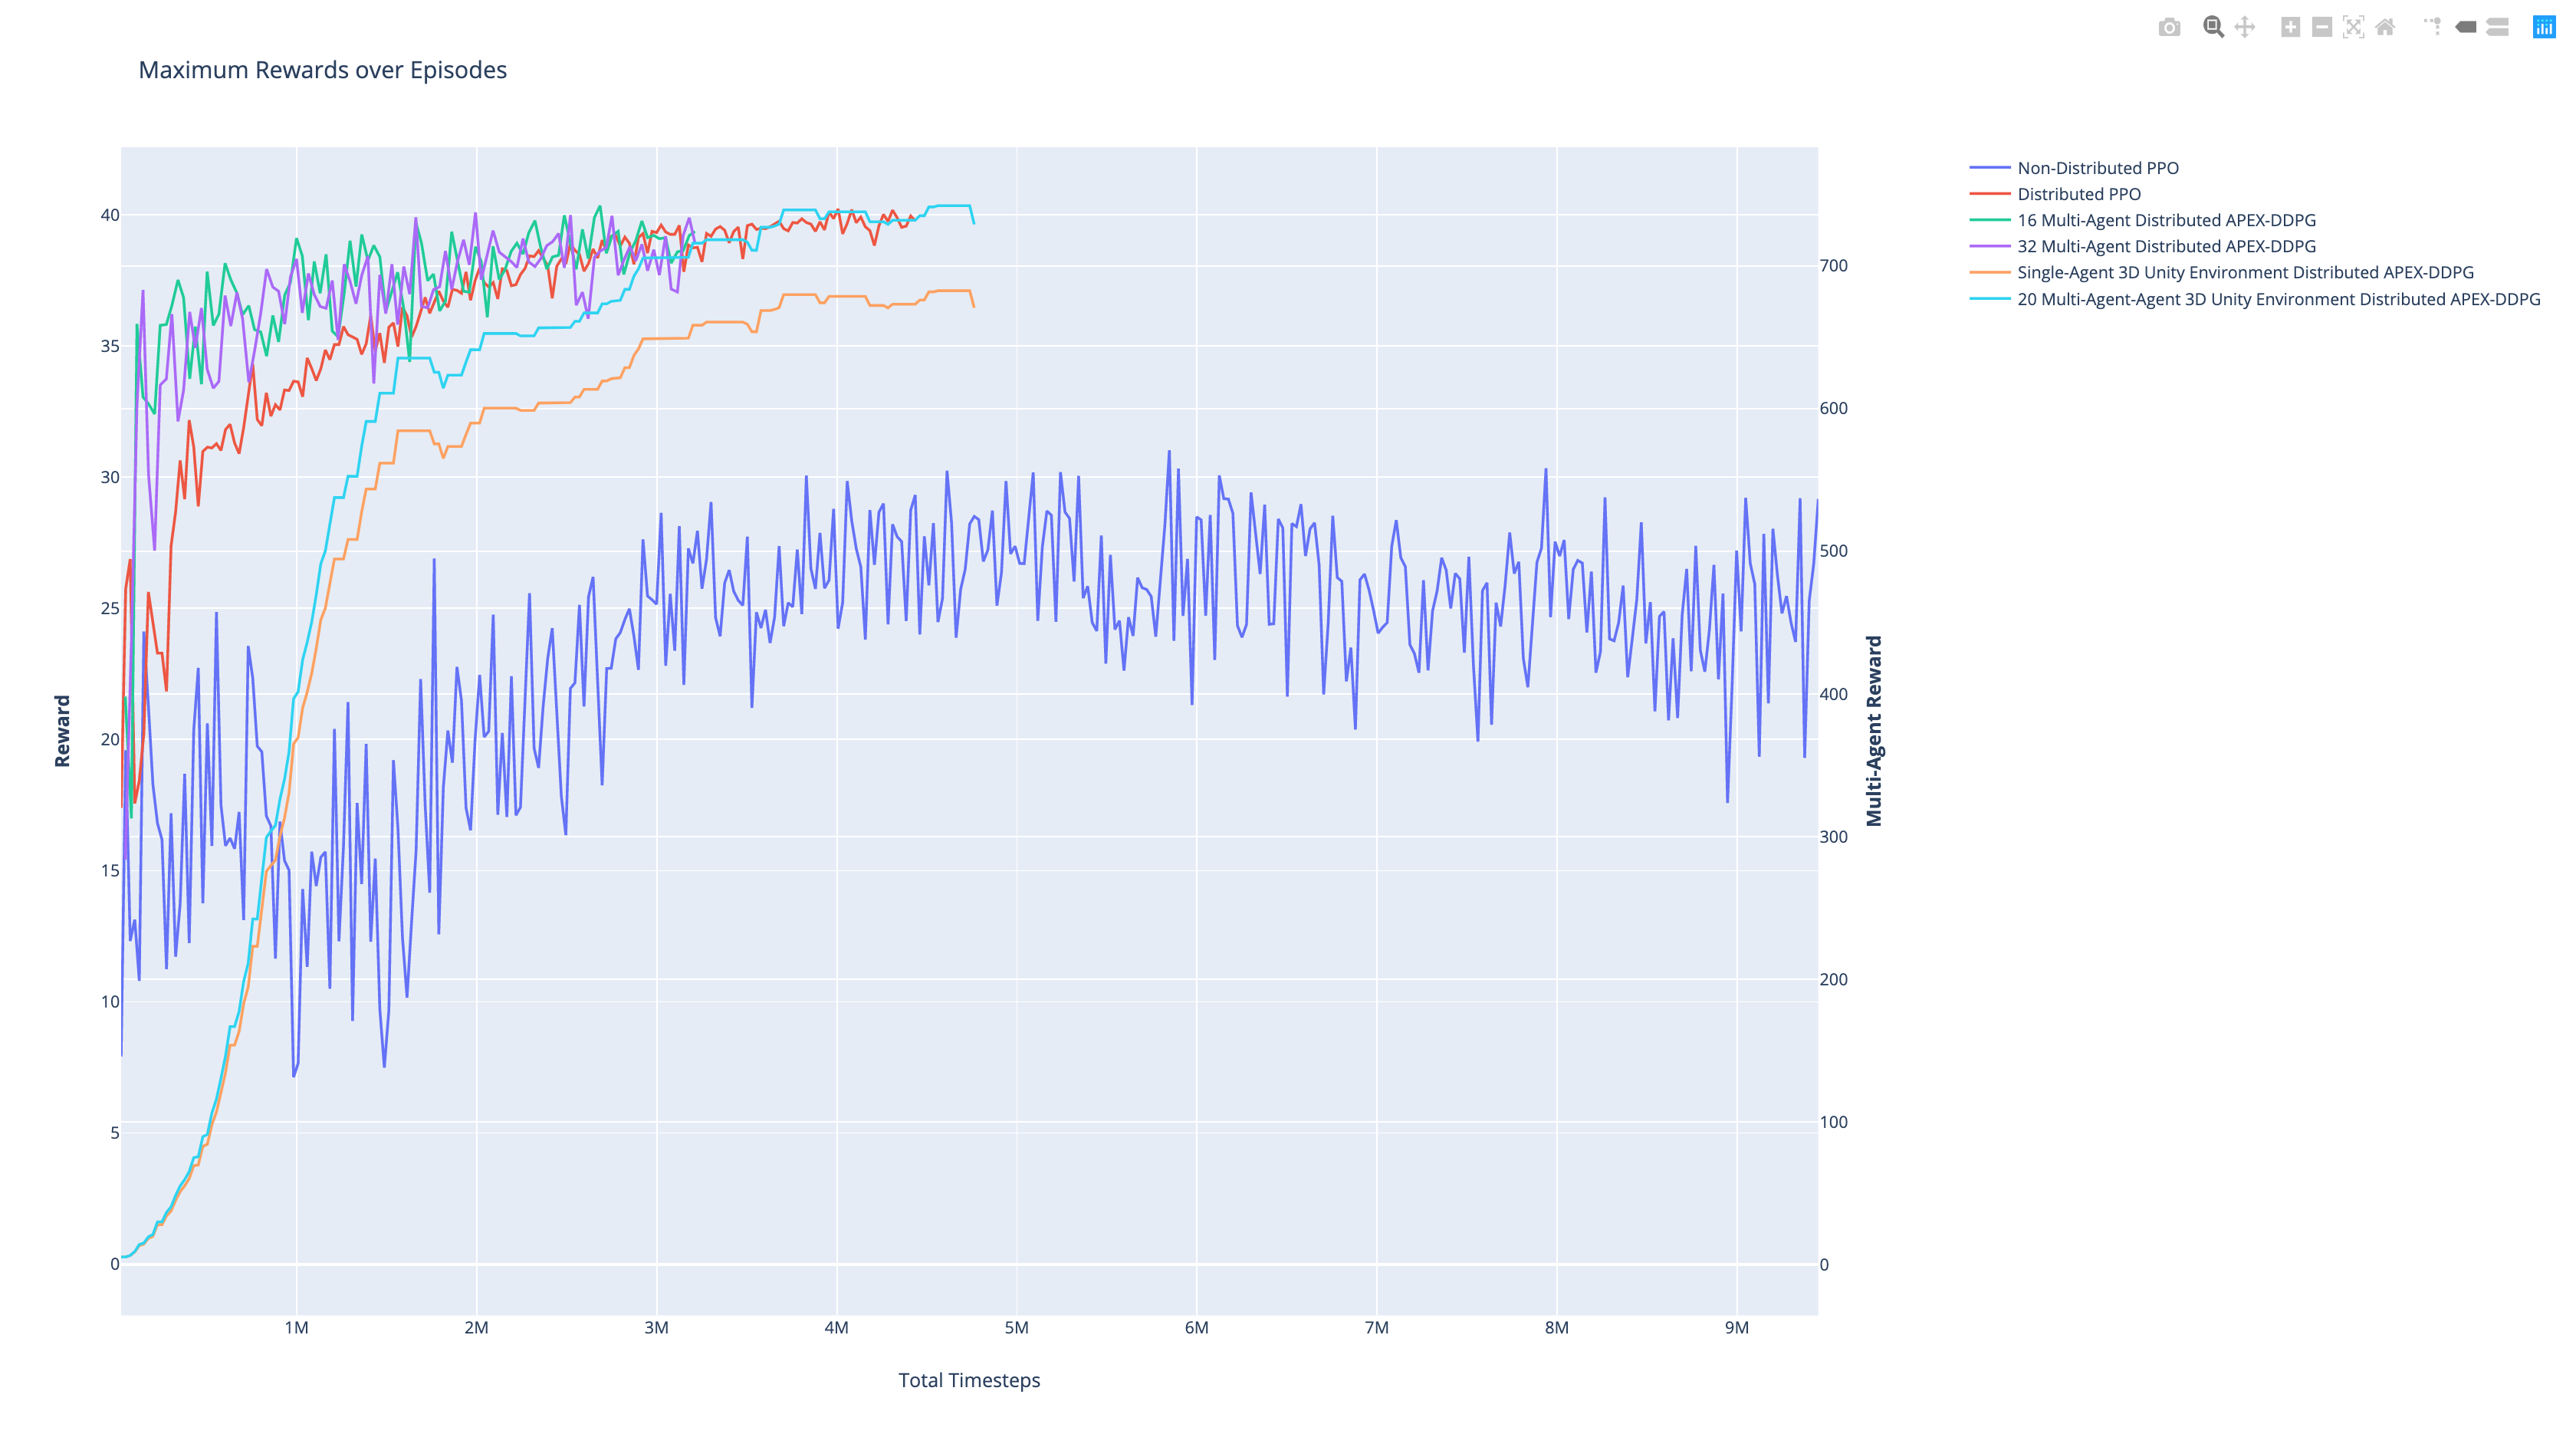
\includegraphics[width=0.8\linewidth]{figures/exps/4th_exp/max_eps_reward.png}
		\caption{Maximum Reward over Episodes}
		\label{fig:4th_exp_max_eps_reward}
\end{figure}

Since the experiments are constrained under the conditions of reaching average reward of 21 or completing 10M steps, we compare the performance of both agents for the average reward. The observation are the distributed version of the agent exceed the average reward obtained by the non-distributed agent after only 500,000 time-steps. Followed by performance improvement over time-steps as the agent reach 15 reward after 2M time-steps, and reaching 20 reward after 4M time-steps, leading the agent to solve the environment and achieve the specified 21 average reward after 6M time-steps only. Hence, the agent performance is better than the previous one and could solve the environment effectively before reaching 10M time-steps. The following figure~\ref{fig:3rd_exp_avg_eps_reward}, illustrate the performance of each agent for obtaining the average rewards.
\begin{figure}[!htb]
		\centering
		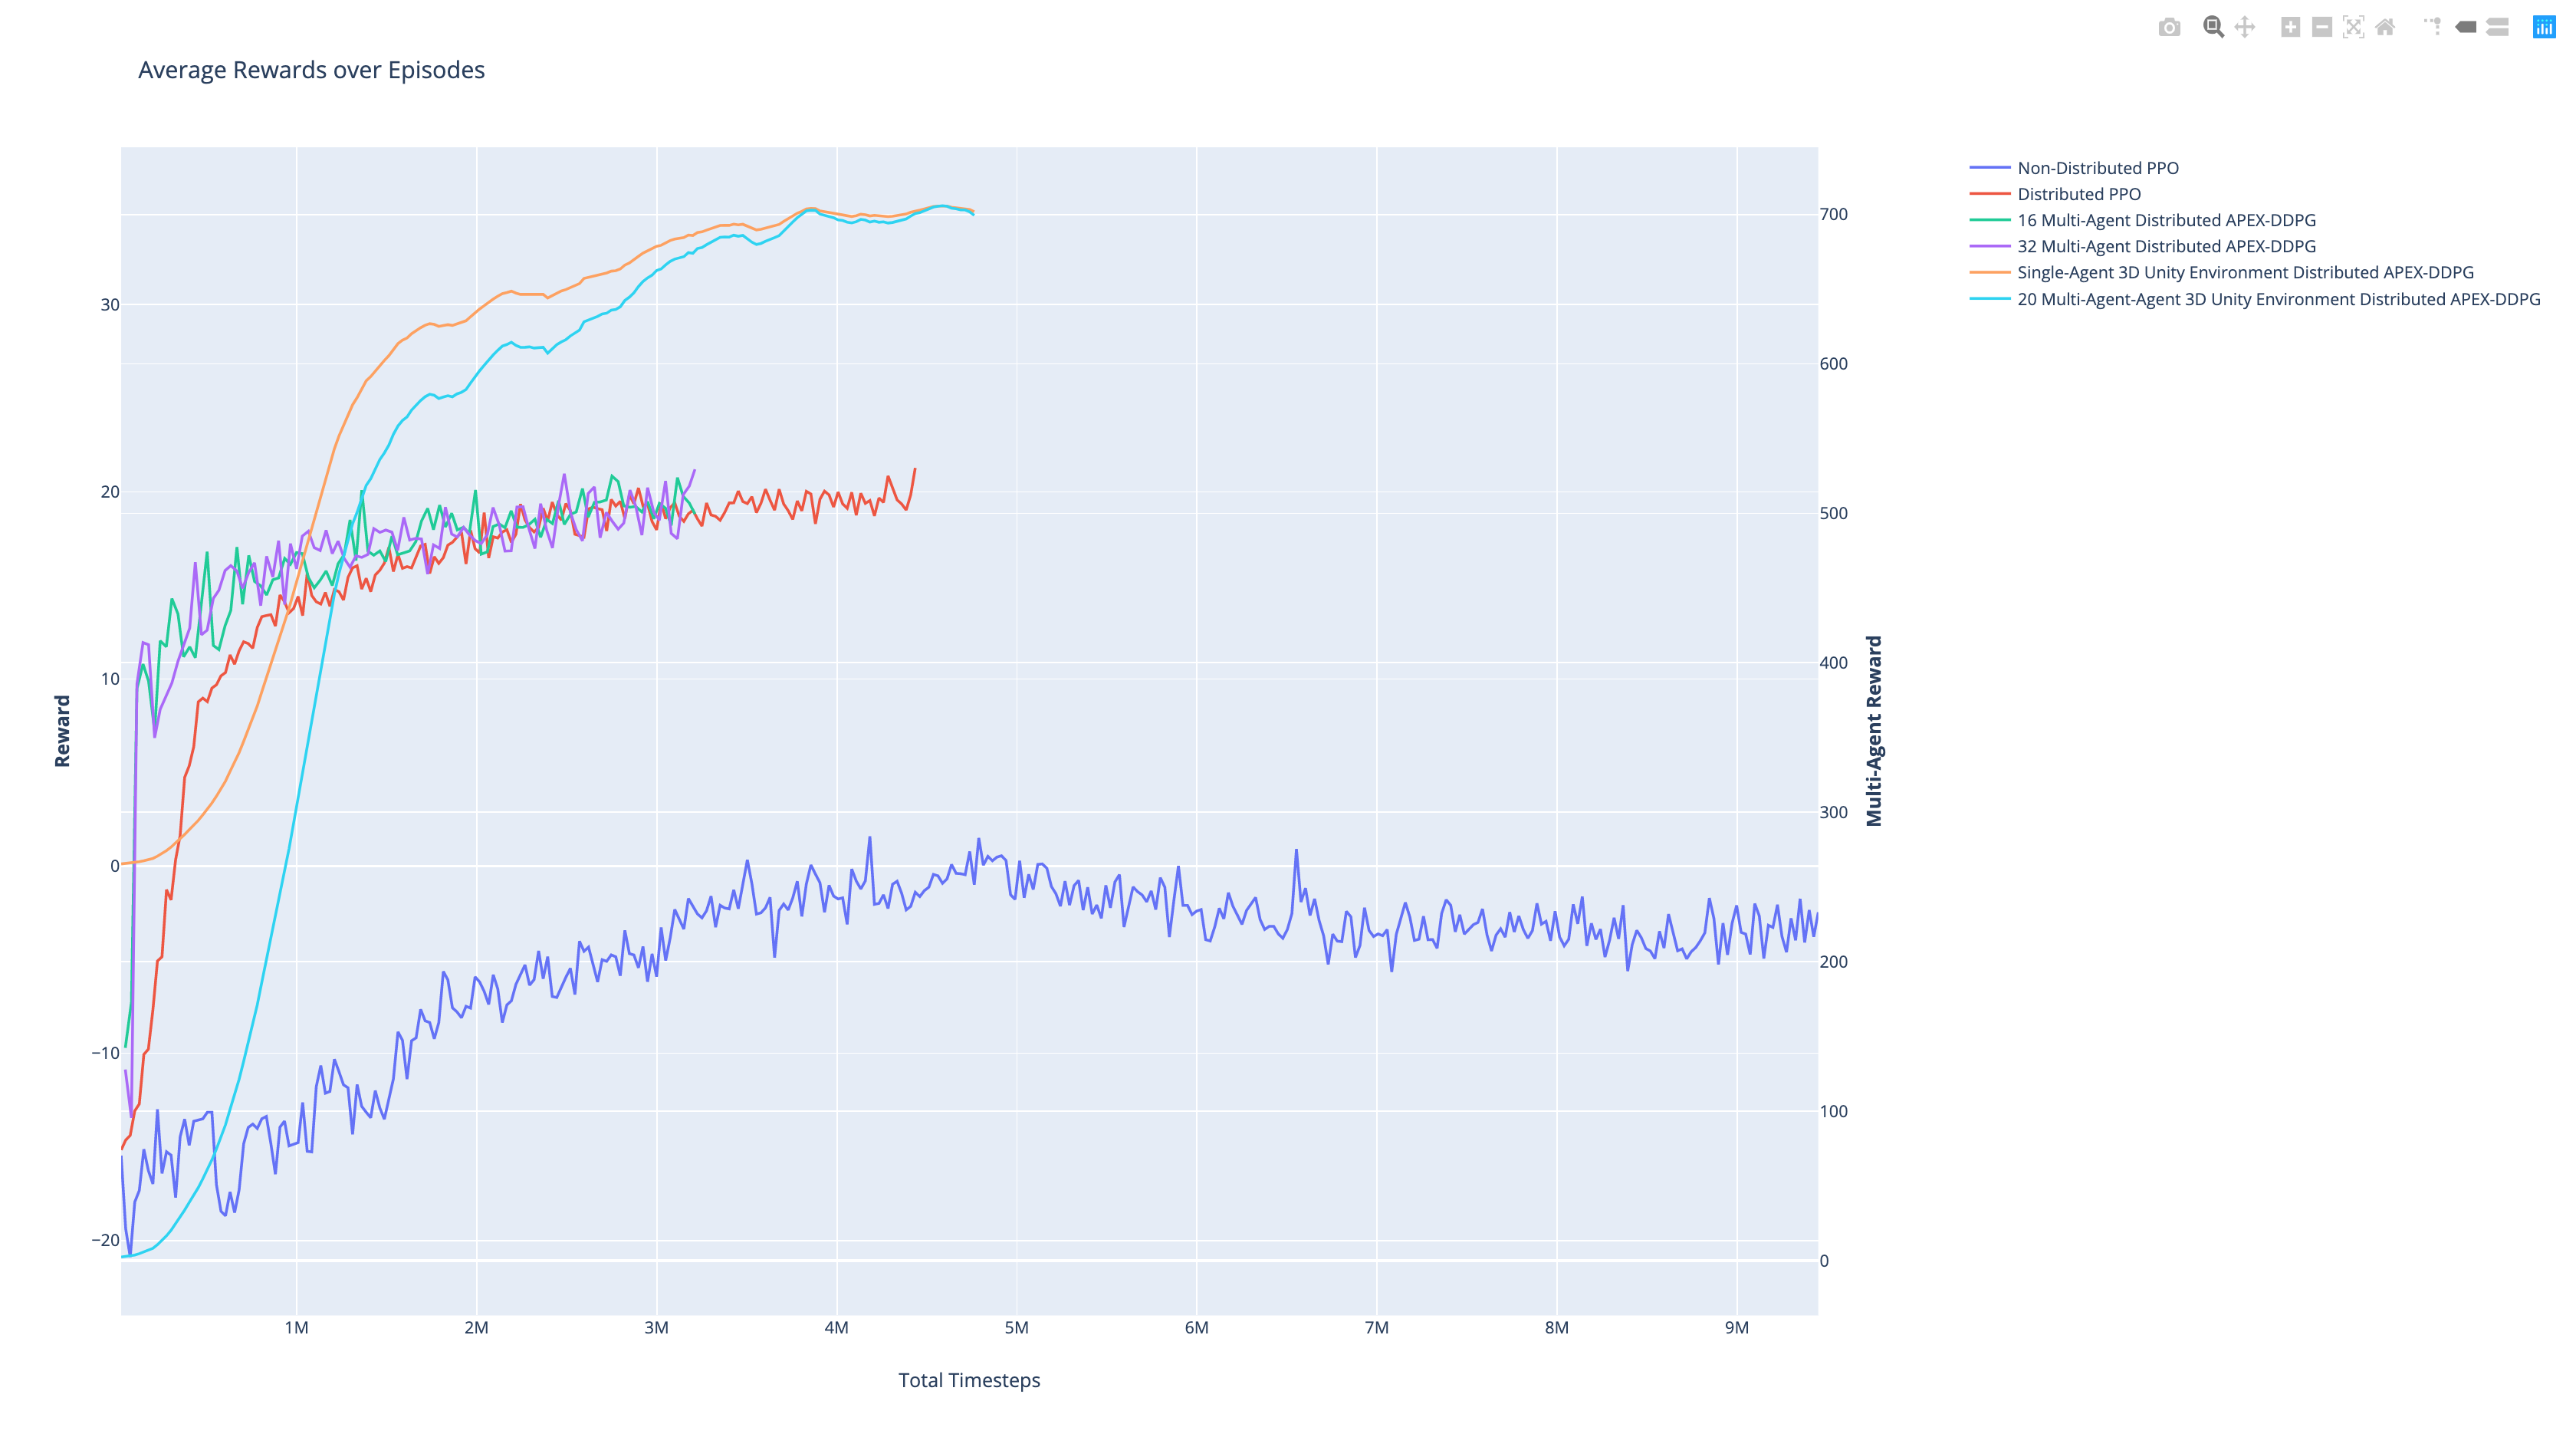
\includegraphics[width=0.8\linewidth]{figures/exps/4th_exp/avg_eps_reward.png}
		\caption{Maximum Reward over Episodes}
		\label{fig:4th_exp_avg_eps_reward}
\end{figure}

Comparing between the experiment's total taken time is crucial as it's one of the main key concept for our experiments. Running the two experiments multiple times with different seeds, we observe that the distributed experiment take half the time needed to perform the non-distributed experiment, making it much faster to train and execute reinforcement learning algorithms in distributed setup. The following figure~\ref{fig:3rd_exp_total_training_time} show the time taken for each experiment per hour.
\begin{figure}[!htb]
		\centering
		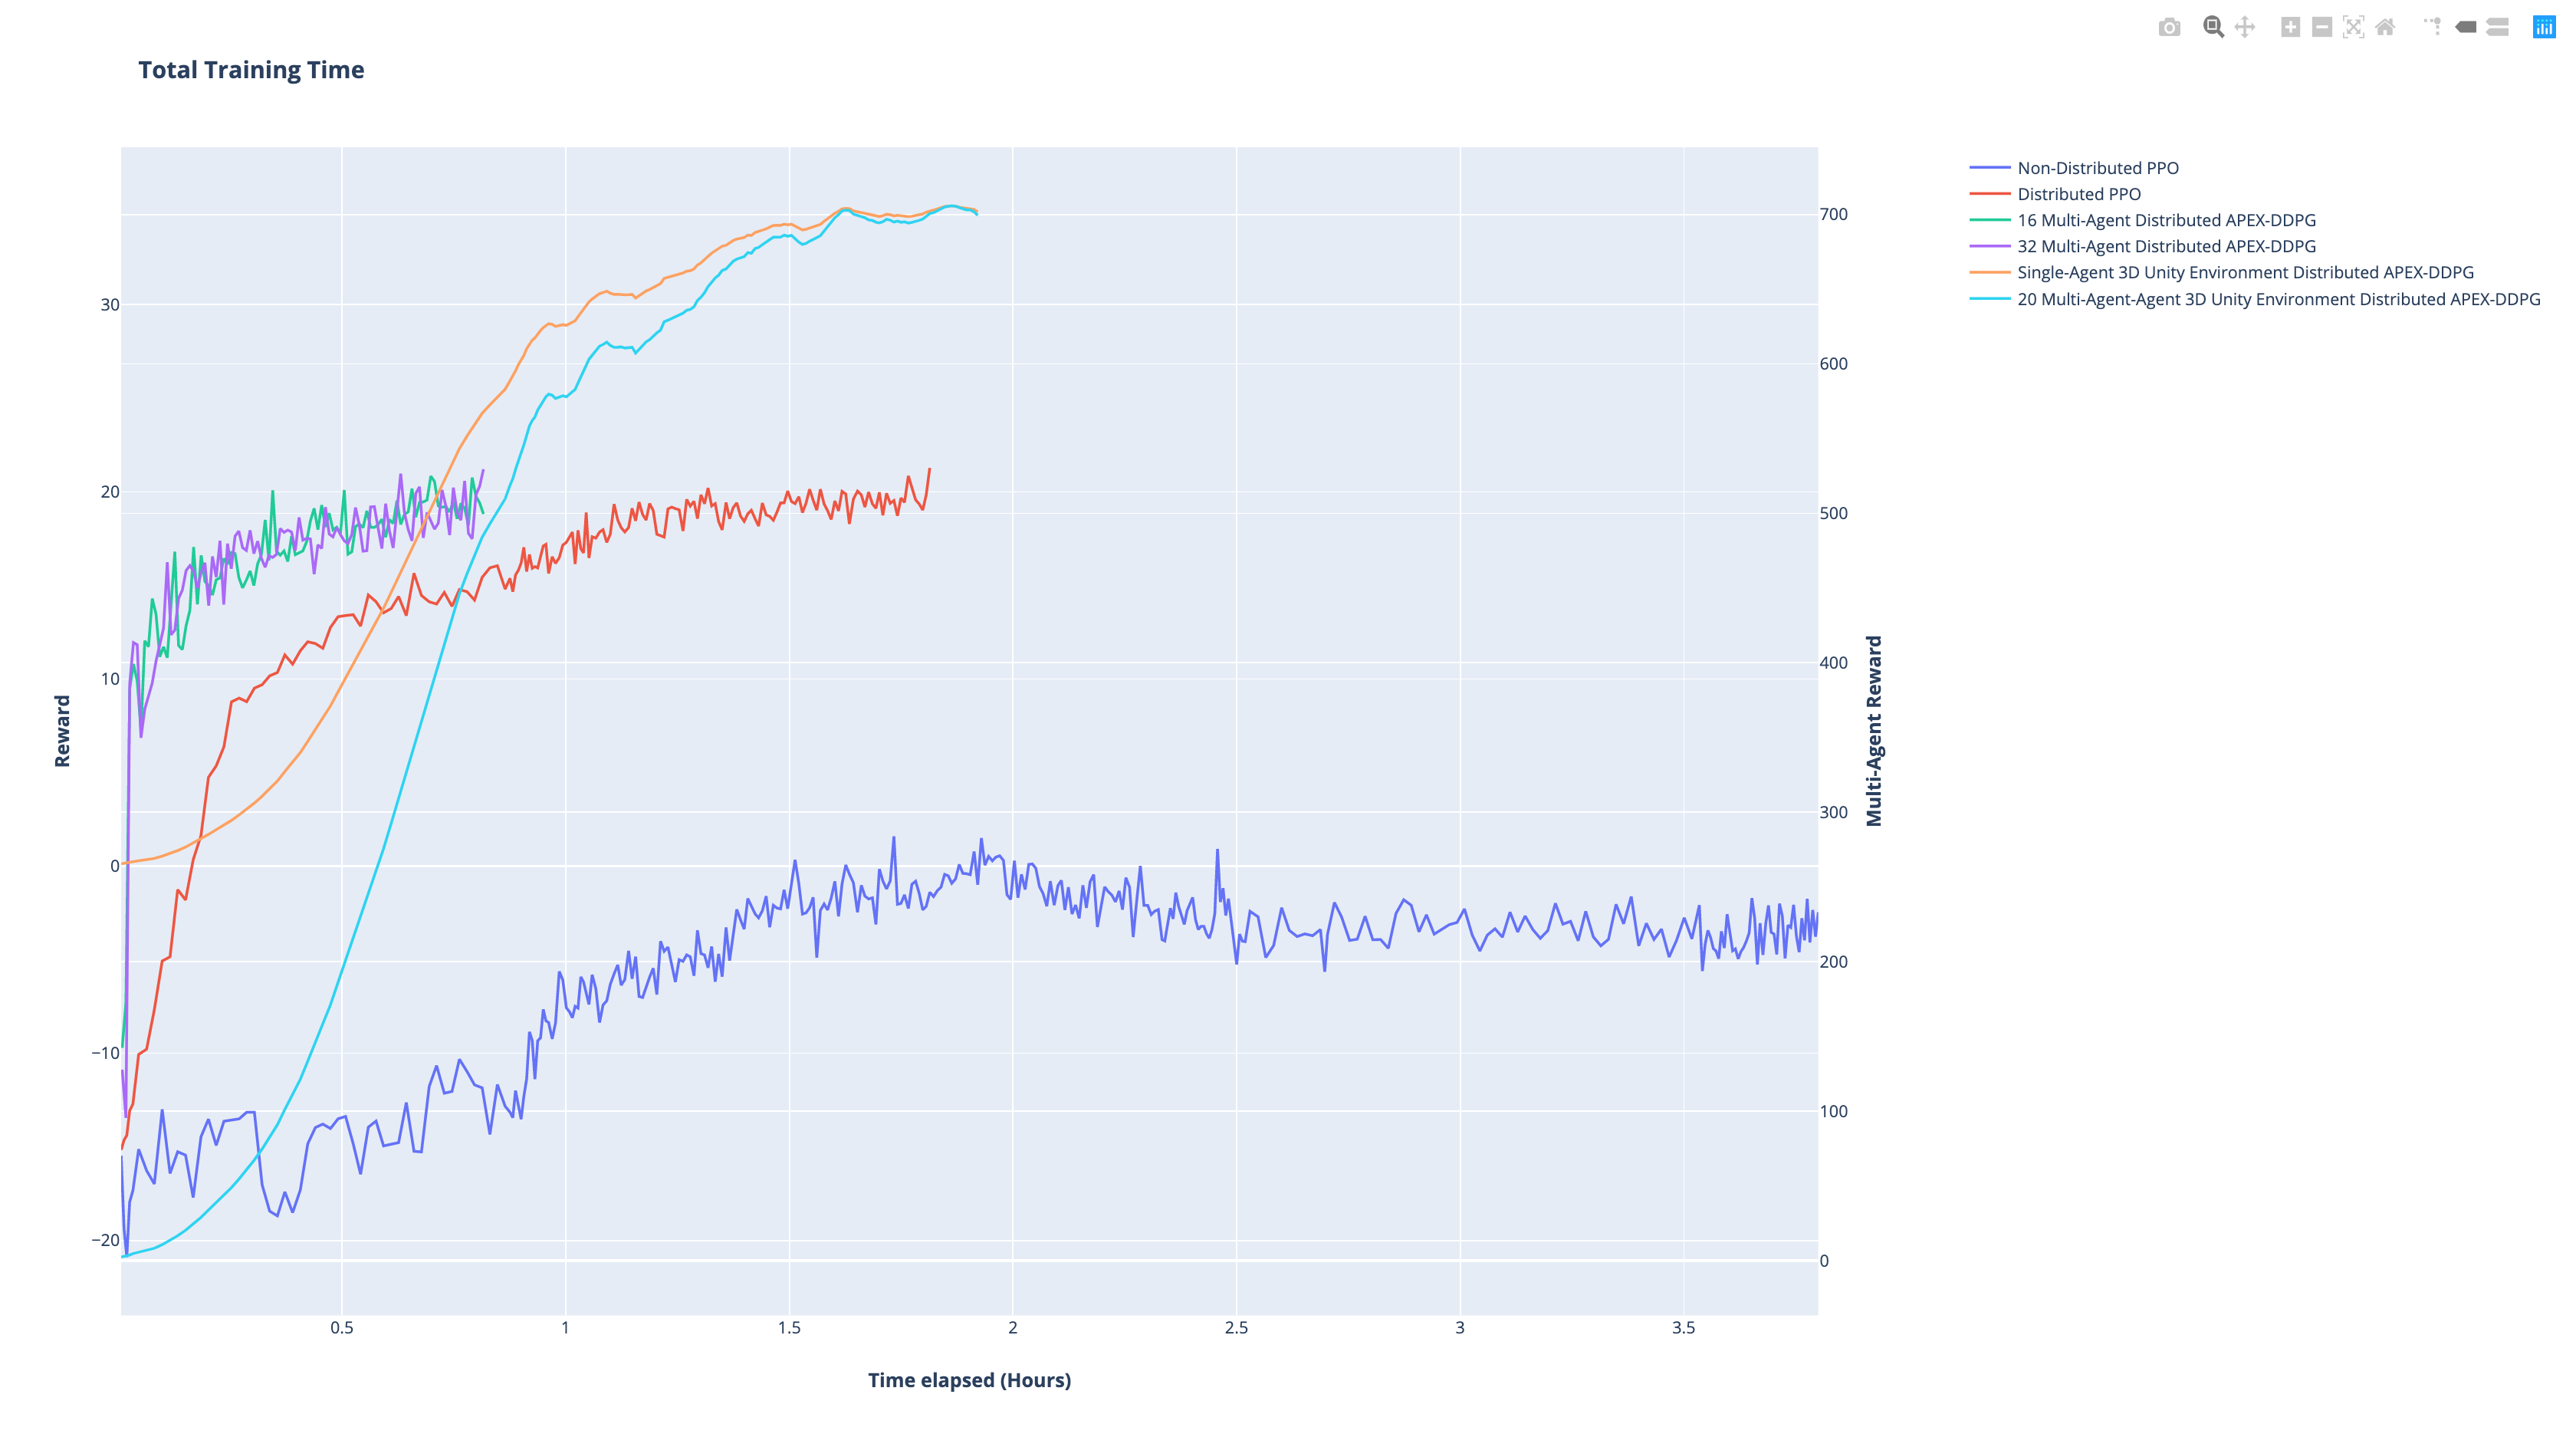
\includegraphics[width=0.8\linewidth]{figures/exps/4th_exp/total_training_time.png}
		\caption{Total Training Time}
		\label{fig:4th_exp_total_training_time}
\end{figure}

$\bullet$ \textit{Second Trail: Transfer learning from gym trained agent} in this experiment, the agent was trained on the previous environment with a modification for the neural network used to train the agent to share the same number of observation and action spaces. After training the agent, it was evaluated on the unity environment to observe how the agent will behave.

Based on the evaluation the agent wasn't able to achieve any reward as shown in the figure below. This is because the agent was trained to output actions that are applied to the Y-axis in gym environment to be able to move the arm correctly. In contrast, unity environment applis the actions to X and Z axes for the arm.
\begin{figure}[!htb]
		\centering
		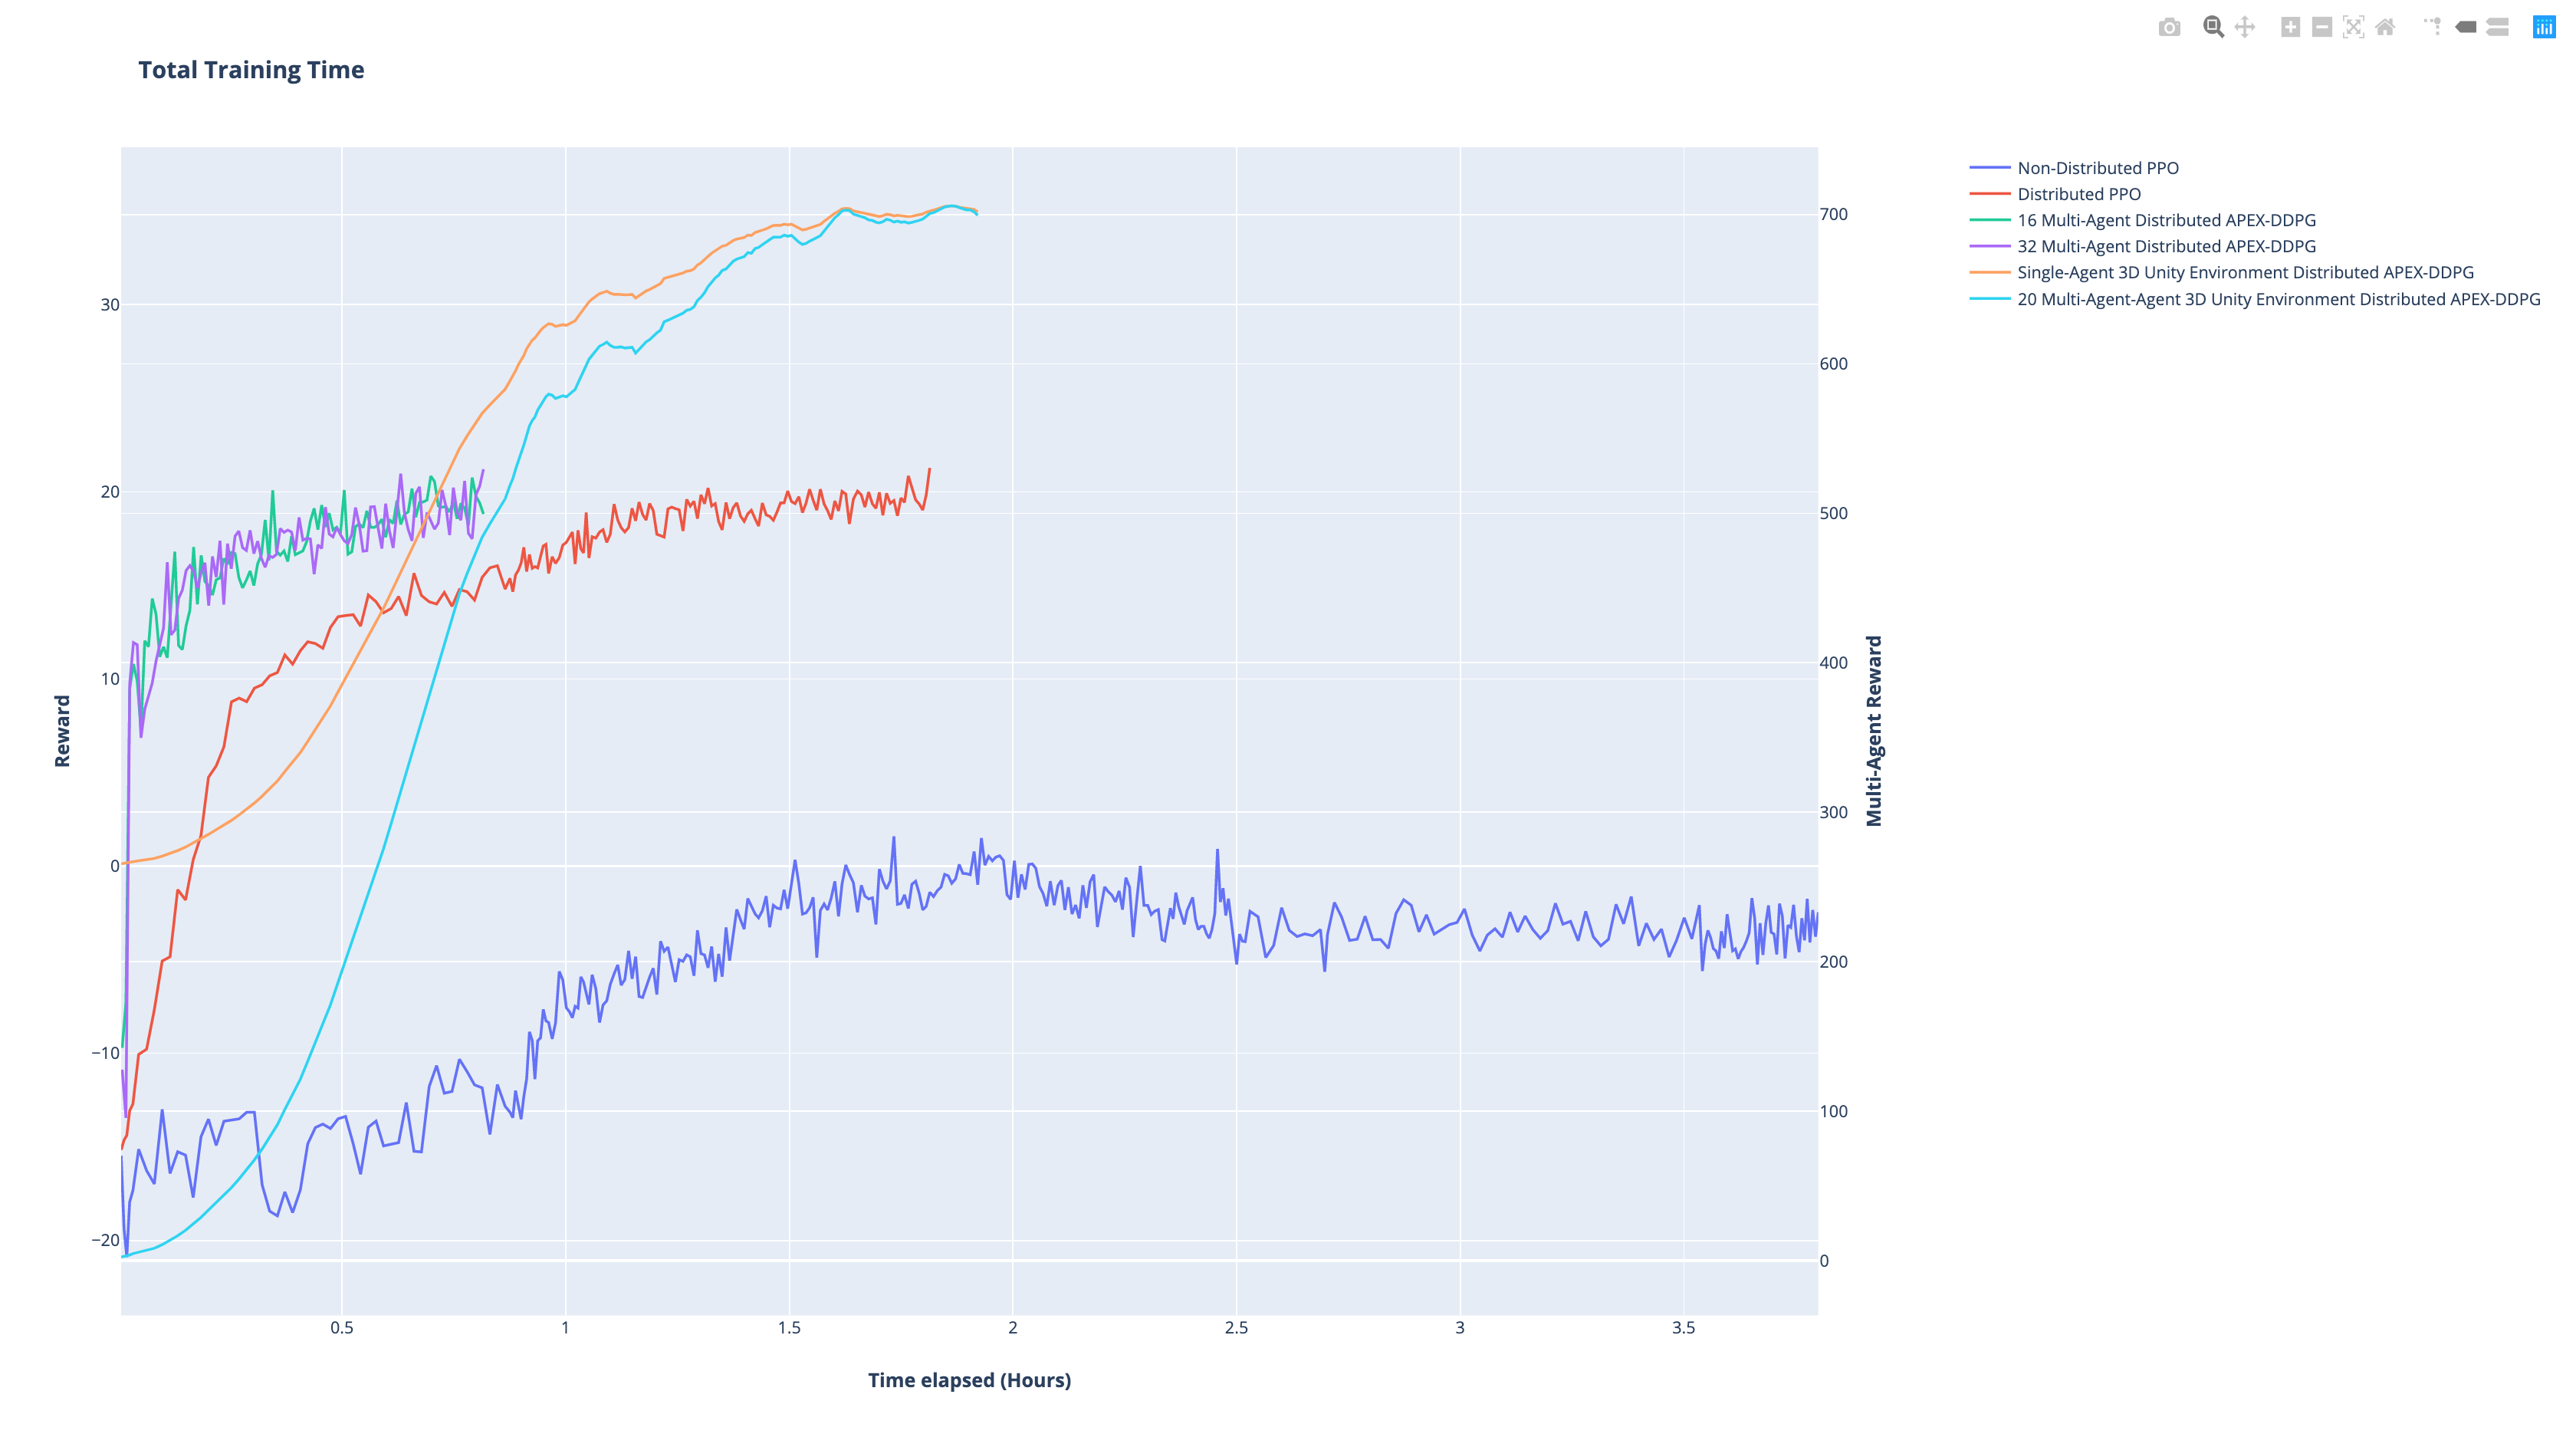
\includegraphics[width=0.8\linewidth]{figures/exps/4th_exp/total_training_time.png}
		\caption{Total Training Time}
		\label{fig:4th_exp_total_training_time}
\end{figure}

In order to benefit from the trained agent, the experiment continue training the agent with unity environment and using the pretrained weights and model from the gym trained agent to accelerate the training of the agent in the new environment. After only 10 minutes as shown in the figure below, the agent was able to move the arm correctly and collect +25 reward based on the running evaluation on 1M time-steps.
\begin{figure}[!htb]
		\centering
		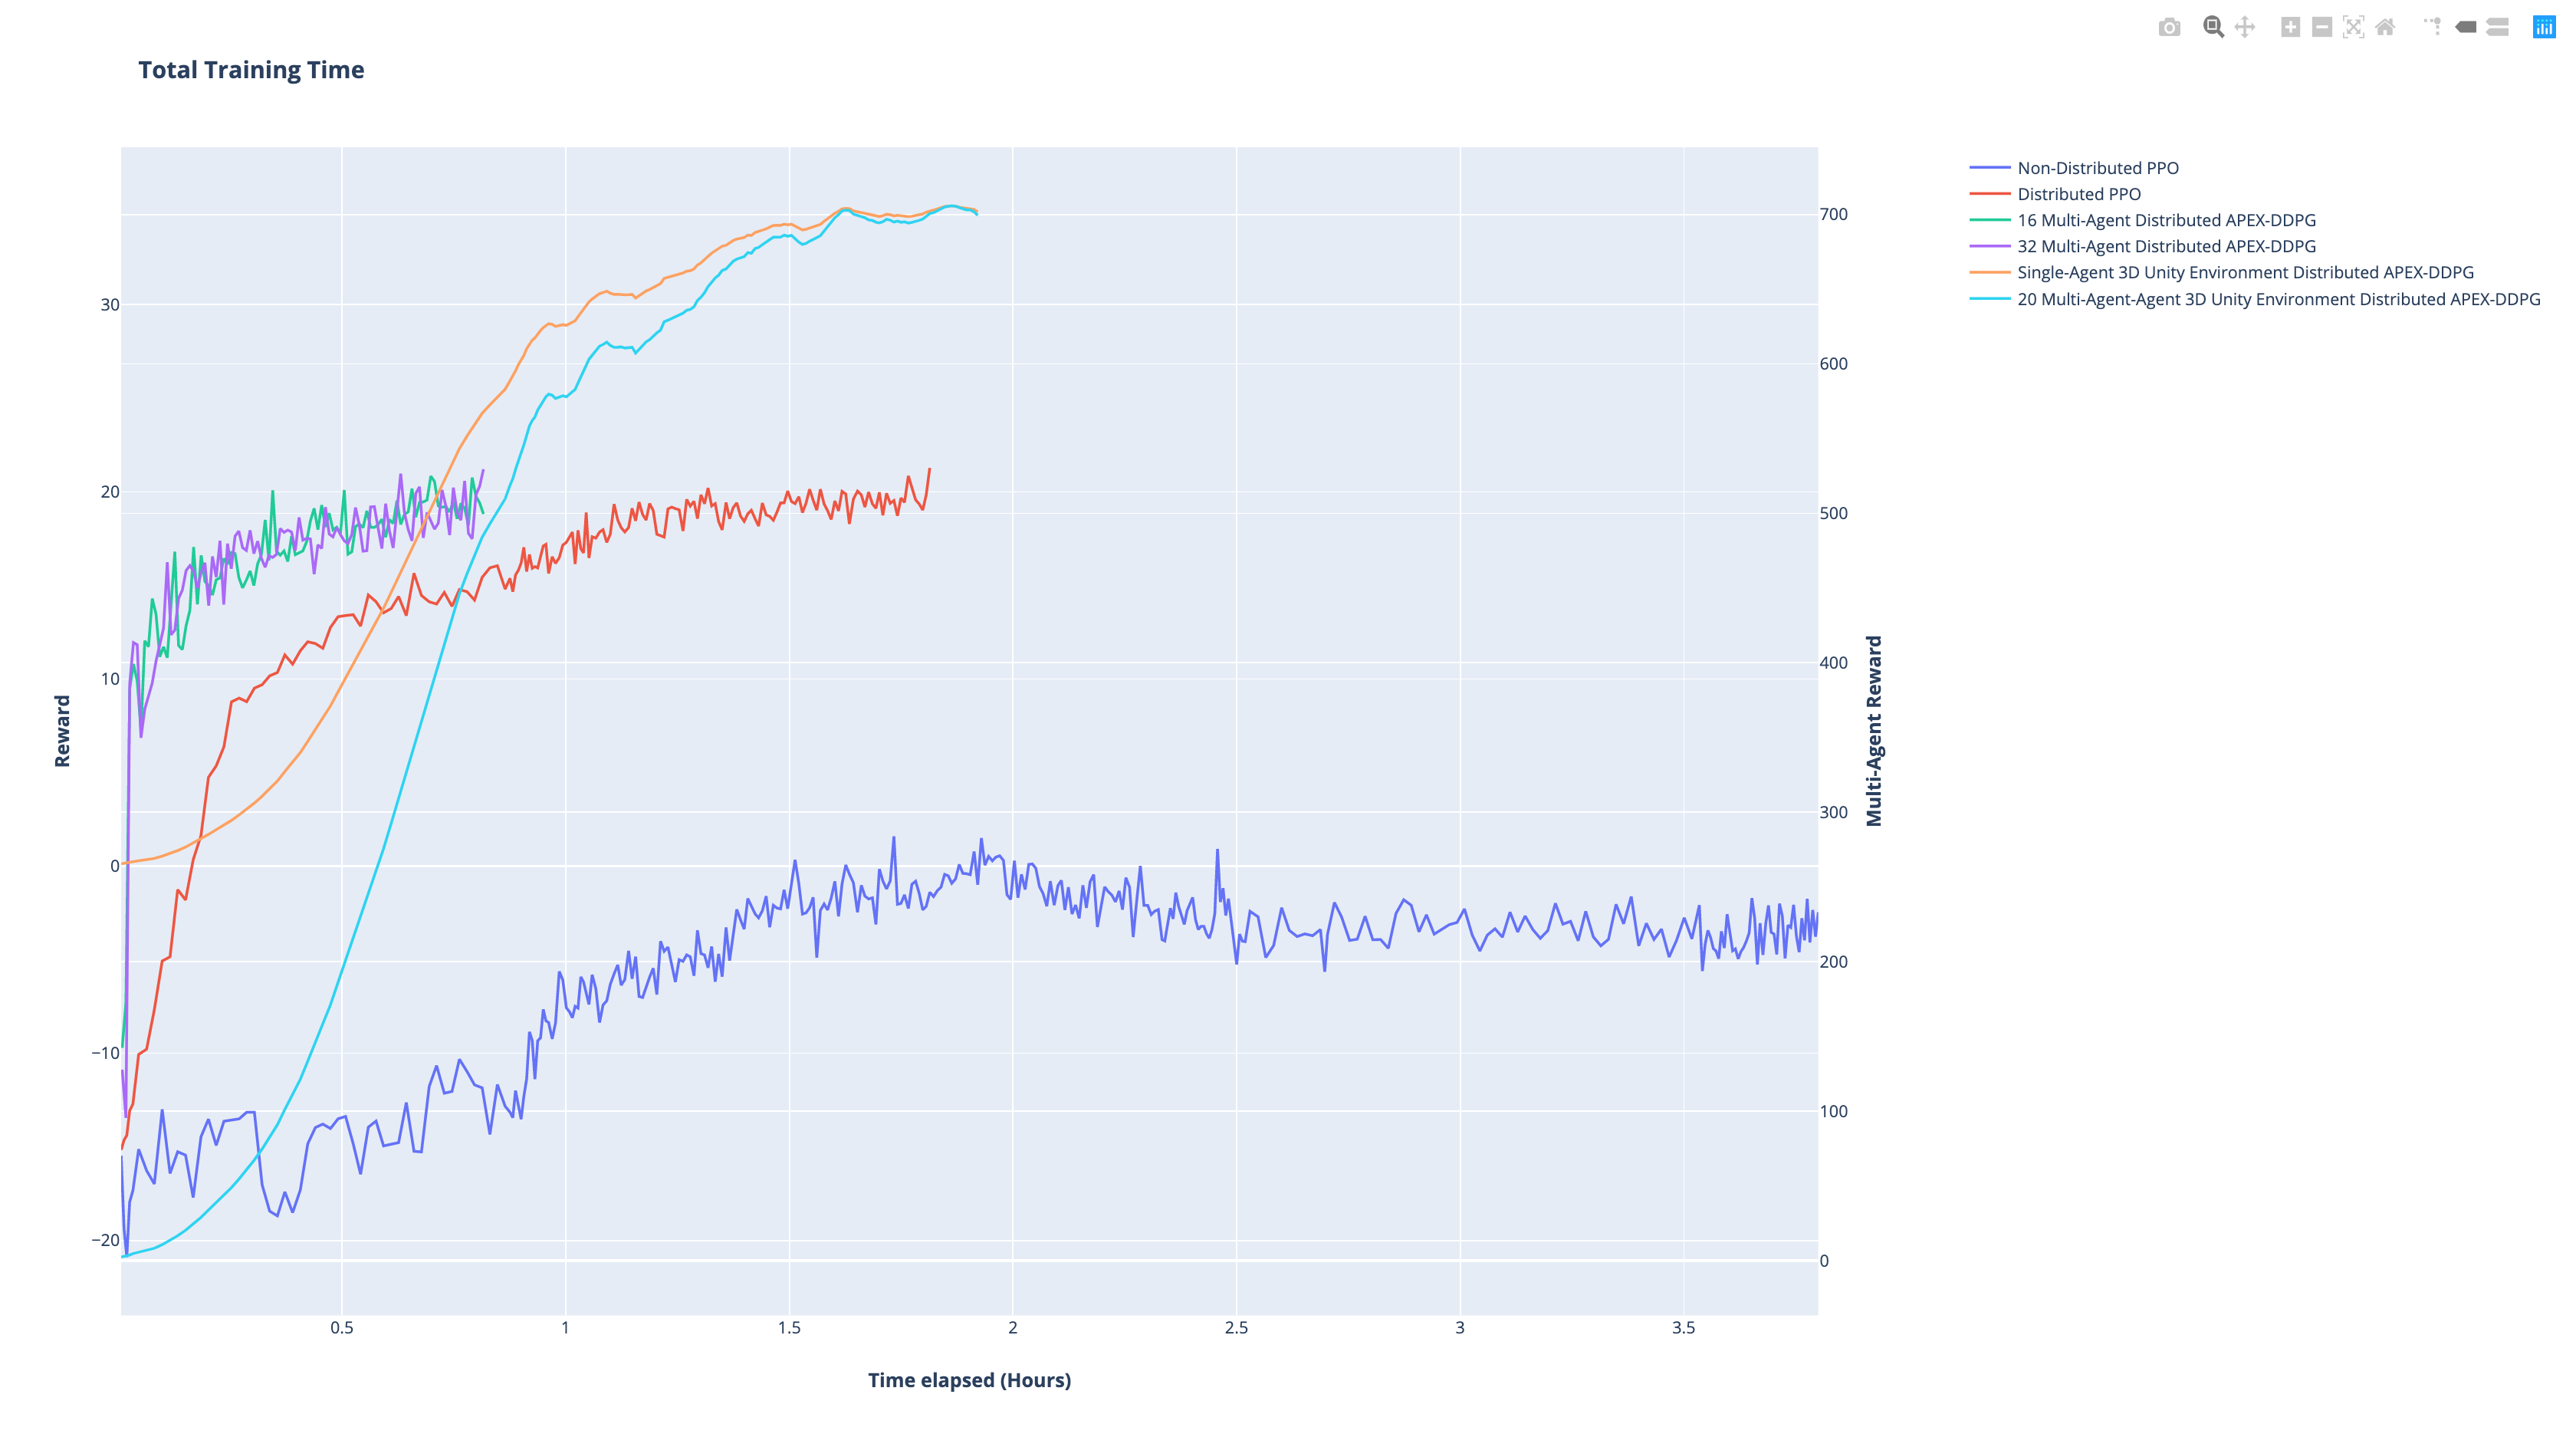
\includegraphics[width=0.8\linewidth]{figures/exps/4th_exp/total_training_time.png}
		\caption{Total Training Time}
		\label{fig:4th_exp_total_training_time}
\end{figure}



\subsubsection{Conclusion}

In this experiment, we perform a training and evaluation for the simple robotic task using ppo algorithm in non-distributed setup to train our agent. we conclude that the experiment took a large amount of time to train the agent (4 hours) and at the end the agent didn't solve the required task and the learning process was not successful. 